%*******************************************
\section{Target Group}
%*******************************************
\label{s:target_group}
This chapter deals with the target group we want to address with our app.
After defining our target audience we briefly explain how it can be projected to the German population.

\subsection{Target Group Definition}
\label{s:target_group_def}
In this section we discuss our target audience.
The main condition our target users have to meet is that they can learn something from our app.
This means users who have too much prior knowledge on the topic of phishing will not benefit from our app.
Thus, these users are not addressed by us.
In detail our target group can be modeled with the aid of the conditions listed below.
\begin{description}[leftmargin=0cm]
\item[Attackability:] The first precondition that all of our users have to meet is that they are possible targets for phishing.
Thus, attackability includes a user's disability to detect phishing.
Attackability also includes that the users have to use the Internet frequently so that they have a common trust in the web and usually are willing to enter their personal data~\cite{divsi2012divsi}.
\item[Android Users:] The second precondition is that the users should use an Android smartphone, otherwise they will not be able to use the app on a regular basis.
\item[Language:] The information blocks of our app consist of German texts.
Consequently, the target user should be able to read and understand German texts.
\item[Motivation:] The distribution plan for this app is to publish it on the Google Play Store and hope that users download and install it.
Therefore, the target users must have a general interest in learning to protect themselves.
 According to a study by Deutsches Institut f\"{u}r Vertrauen und Sicherheit im Internet (DIVSI)~\cite{divsi2012divsi}, there exist Internet users who are self-confident regarding their knowledge and ability to protect themselves in such a way that they are not willing to learn anything else.
We will not be able to reach these users.
\end{description}
For our final user study we aspired to recruit participants who hold these preconditions as far as possible.
\autoref{s:representativeness} gives a description on this aspect.

Subsequently, we discuss how our target group can be projected to the German population.

\subsection{Projection to Population}
After defining our target group we now want to make sure that we do not exclude too many potential users.
In fact, the app can only be useful and successful if a reasonable audience is covered.
To prove this we looked at an extensive survey by DIVSI~\cite{divsi2012divsi}.
In this survey the authors first looked at 60 persons in detail and found seven types of Internet users that are depicted in \autoref{fig:divsi_milieus}.
Thereafter, they tried to apply their findings to the German population by interviewing 2,000 representative persons.
\autoref{fig:divsi_kartoffeln} illustrates the percentage share of the seven Internet types they identified in Germany.
We strived to match our preconditions to these Internet types which is described in the following.

\begin{figure}[hHtbp]
\centering
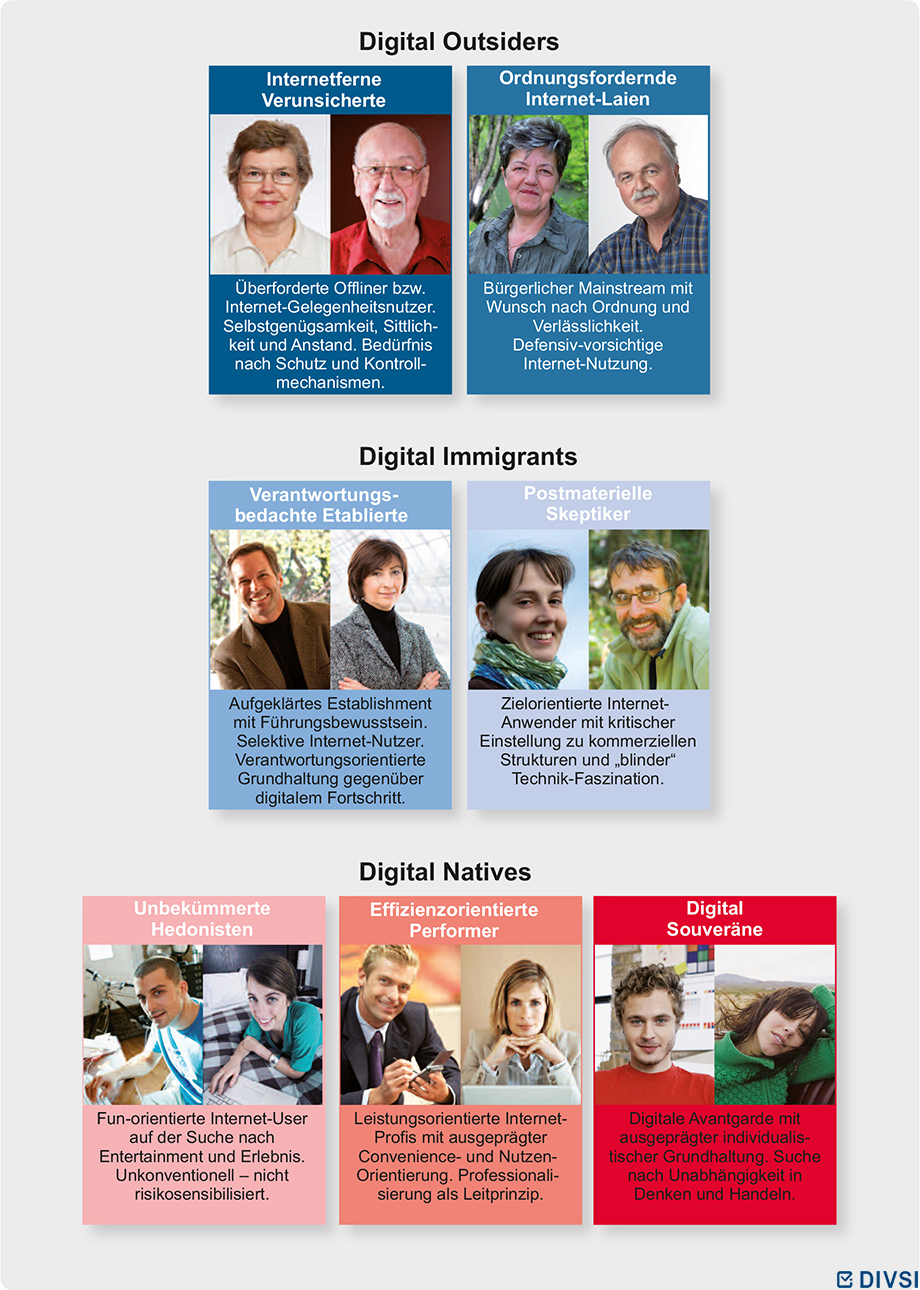
\includegraphics[width=0.9\textwidth]{DIVSI-Milieus.jpg}
\caption{Internet milieus as defined by DIVSI~\cite{divsi2012divsi}}
\label{fig:divsi_milieus}
\end{figure}

\begin{description}[leftmargin=0cm]
\item[Digital Souver\"{a}ne:] This group frequently uses the Internet, and thus is exposed to phishing. Users of this group also usually own a smartphone. However, we have to rule them out because the users of this group are convinced that they already know the problems of the Internet and how to avoid them. Hence, they are unlikely to download our app and  will probably reject any training offer.
\item[Effizienzorientierte Performer:] This group matches our preconditions.
Users of this group frequently use the Internet as well as smartphones. In contrast to the previous group, they are interested in learning something new and see their obtained knowledge as an investment in the future. To reach the users of this group we should show that they can learn something from our app.
\item[Unbek\"{u}mmerte Hedonisten:] This group is also native in the digital world but in contrast to the before mentioned groups, the users of this group are not aware of the problems and frauds therein. In case they are aware of a problem they seek to secure themselves with the aid of automated software instead of dealing with it themselves. Therefore, the users of this group are not likely to be motivated to use our app.
\item[Postmaterielle Skeptiker:] This group is interested in the Internet and uses it frequently. Its users are aware of the problems and frauds raised by the Internet. As they are interested in information on the Internet, especially from official sources, they might download our app. To reach the users of this group we should clearly state that our app originates from a university.
\item[Verantwortungsbedachte Etablierte:] This group is regulary online and also uses smartphones. Its users are especially interested in using protection software and actively seek for information on the Internet. They do not believe that they could protect themselves against the dangers of the Internet and actively aspire to change this. Therefore, we believe that this type of Internet users are likely to appreciate our app. To reach the users of this group we should clearly state that this app helps protect themselves.
\item[Ordnungsfordernde Internet-Laien:] This group uses the Internet rarely. For this reason, the users of this group are particularly careful when using it and usually do not enter personal data. Besides, they usually do not have smartphones. Thus, it is not likely that they will use our app. 
\item[Internetferne Verunsicherte:] These users do not make use of the Internet at all. Therefore, they are not exposed to phishing threats.
\end{description}
\begin{figure}[hHtbp]
\centering
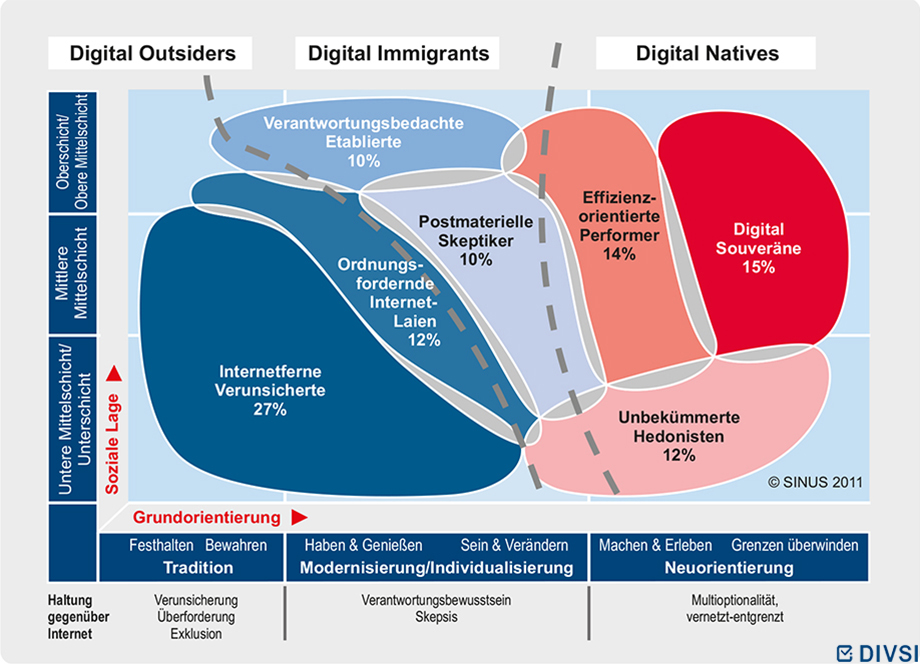
\includegraphics[width=0.6\textwidth]{DIVSI-Kartoffeln.jpg}
\caption{Internet milieus projected to German population~\cite{divsi2012divsi}}
\label{fig:divsi_kartoffeln}
\end{figure}
To sum it up, we consider the Internet user types of \textit{Verantwortungsbedachte Etablierte} (10\%),  \textit{Postmaterielle Skeptiker} (10\%), and \textit{Effizienzorientierte Performer} (14\%). In total these groups represent 34\% of the German population.